%%%%%%%%%%%%%%%%%%%%%%%%%%%%%%%%%%%%%%%%%%%%%%%%%%%
%
%  New template code for TAMU Theses and Dissertations starting Fall 2012.  
%  For more info about this template or the 
%  TAMU LaTeX User's Group, see http://www.howdy.me/.
%
%  Author: Wendy Lynn Turner 
%	 Version 1.0 
%  Last updated 8/5/2012
%
%%%%%%%%%%%%%%%%%%%%%%%%%%%%%%%%%%%%%%%%%%%%%%%%%%% 

%%%%%%%%%%%%%%%%%%%%%%%%%%%%%%%%%%%%%%%%%%%%%%%%%%%%%%%%%%%%%%%%%%%%%%%
%%%                           SECTION II 
%%%%%%%%%%%%%%%%%%%%%%%%%%%%%%%%%%%%%%%%%%%%%%%%%%%%%%%%%%%%%%%%%%%%%%%

\chapter{  \uppercase {constitutive model for polarization switching}  } 
\label{section:chap_02_constitutive_model_for_polarization_switching}

This chapter deals with macroscopic response of materials that possess electro-mechanical coupling behaviors,
 focusing on piezoelectric ceramics of Perovskite structures. 
The macroscopic response of the materials strongly depends on their
microstructural changes when they are subjected to external stimuli.
A single crystal of Perovskite undergoes a spontaneous polarization, indicating
by a separation of negative and positive charges, at temperatures below its Curie temperature. 
This separation is quantified by a dipole moment and a dipole moment per unit volume is known as polarization. 
The direction of the polarization in this crystal structure is towards the positive charge. 
As bulk piezoelectric ceramics comprise of polycrystalline structures,
 the spontaneous polarization axes of all crystalites are
 randomly distributed upon processing the piezoelectric ceramics. 
Therefore, net (macroscopic) polarization is considered zero and the materials do not show macroscopic electro-mechanical coupling response. 
Applying an electric field in certain direction would align the poling directions of the crystallites towards the electric field direction so that the net polarization of the materials is measurable,
 as illustrated in figure \ref{fig:Majorhysteresisloops}a, where $x_3$ is the direction of the electric field applied. 
Increasing the electric field would increase the measured polarization untill it
reaches the saturated value and upon removal of the electric field, there exist a remanent polarization\footnote{The ability of materials to undergo spontaneous polarization and retain its polarized state after removal of electric field is called ferroelectricity.
 The materials with ferroelectric behavior are called ferroelectric materials.}. 
The net poling axis of the piezoelectric materials can be reversed by applying an electric field in the opposite direction to the current polarization. 
When the net polarization in the materials is non-zero the materials have electro-mechanical coupling responses,
 as shown by the corresponding nonzero strain in figure \ref{fig:Majorhysteresisloops}b, which shows a strain response with respect to the applied electric field.


For practical application purposes, the materials need to be polarized/poled in order to have an electro-mechanical coupling. 
This is done by applying a relatively large electric field, greater than the coercive electric field ($E_c$) of the material,
 until it reaches the saturated polarization,
  which is often done at elevated temperatures but below the Curie temperature of the material \cite{Lines1977},
   then the temperature is decreased to room temperature prior to removing the electric field which results in a remanent polarization. 
At this stage, the polarized material would have piezoelectric effects, as shown by the minor loops in figure \ref{fig:Manorhysteresisloops}a,b. 
By applying an electric field, the polarized material would undergo mechanical deformations or experience stresses and when a mechanical load is applied the polarized material would generate electric charge or voltage difference. 
Typically, electric fields and/or mechanical stresses should be applied to the piezoelectric materials with their magnitude less than the coercive limit so that they will not cause depolarization of the materials. 
Applying large electric field or compressive stress in the poling direction to the polarized materials would cause depolarization and  consequently loss of the electro-mechanical coupling properties. 
The stress and electric field threshold that causes depolarization are called coercive stress and coercive electric field, respectively\cite{Sohrabi201344}.

Polarization behaviors in the materials due to application of cyclic electric fields show hysteretic responses (see figure \ref{fig:Majorhysteresisloops} and figure \ref{fig:Manorhysteresisloops}). 
These responses also depend on the frequencies of the electric field inputs, ambient temperatures, and existence of mechanical loading. 

\section{Phenomenological Model}
A time-dependent hysteretic polarization model is formulated to describe the macroscopic polarization response of ferroelectric materials
 due to various histories of external electric field inputs. 
The model is then modified to include the effect of the mechanical stress on the
 polarization response of the ferroelectric materials \cite{Muliana2011,Sohrabi201344}.
Consider an electric field input in the $x_3$ direction $E_3(s),s>0$,  and $E_3(s)=0,\forall s<0$  , where $s$ is the time history.  
The corresponding polarization response at current time $t$ is:

\begin{equation}
P_3^t\equiv P_3[E_3(t-s),t]=R[E_3(t-s),t]+Q[E_3(t-s),t]
\label{EQN:polarization_decomposition}
\end{equation}
where $R[E_3(t-s),t]$ is the time-dependent reversible polarization response at current time $t\geq 0$ with $R[0,t]=0$ and $Q[E_3(t-s),t]$ is the residual (irreversible) polarization. The reversible polarization response is expressed as:

\begin{equation}
\label{EQN:RevPol}
R^t\equiv R[E_3(t-s),t]= R[E_3^0,t]+\int_{0^+}^t\frac{\partial R}{\partial E_3} [E_3^t,t-s] \frac{dE_3^s}{ds}ds , t \geq 0
\end{equation}

\begin{equation}
R[E_3^0,t]=R_0(E_3^0)+R_1(E_3^0)\big(1-exp\bigg[-\frac{t}{\tau_1}\bigg] \big)
\label{EQN:StaticRevPol}
\end{equation}

One may consider $R[E_3^0,t]$ as the polarization at current time $t$ due to a constant electric field applied at $s=0$. 
The superscript $s$ and $t$ denote the representative of the previous time history and current time, respectively.
 Both $R_0(E_3^s)$ and $R_1(E_3^s)$ are functions of $E_3^s$. The characteristic time $\tau_1$ measures the speed that the polarization changes with time.
 For a linear electric behavior $R_0(E_3^s)$ and $R_1(E_3^s)$ are considered as follows:

\begin{equation}
\begin{aligned}
&R_0(E_3^s)=\kappa_0 E_3^s \\
&R_1(E_3^s)=\kappa_1 E_3^s
\end{aligned}
\label{EQN:R0R1Defini}
\end{equation}
where $\kappa_0$ is the dielectric constant of a macroscopically non-polarized material
 (corresponding to the second order permeability tensor in a multi-axial case) and $\kappa_1$ is the time dependent dielectric constant;
 when $\kappa_1=0$ ,
 a time-independent polarization behavior is considered. 
The state of polarization is defined through the following polarization function:
 
\begin{equation}
\label{EQN:SurfacePol}
f(P_3^t,P_c)=\left< {P_3^t}^2-P_c^2 \right> 
\end{equation}
where $P_c$ is the current polarization state,
 analogous to yield stress in an over stress plasticity theory,
  and $<>$ are the Macaulay brackets.
It is assumed that the irreversible polarization is formed when $f(P_3^t,P_c)=0$ and $E_3^t P_3^t>0$. 
The irreversible polarization is defined as:

\begin{equation}
Q^t\equiv Q[E_3^t]= \int_{0^+}^{E_3^t}\frac{d Q^s}{d E_3}{dE_3}
\label{EQN:IrrevePol}
\end{equation}

\begin{equation}
\frac{d Q^t}{d E_3}=
\begin{cases}

\lambda|\frac{E_3^t}{E_c}|^n & \text{if } |E_3^t|\leq E_c, f=0 \\
\mu \times exp[-\omega(\frac{|E_3^t|}{E_c}-1)] & \text{if }|E_3^t|> E_c, f=0 \\ 0
& \text{if } f \leq 0 

\end{cases}
\label{EQN:TimeDepIrrevePol}  
\end{equation}
where $E_c$ is the coercive electric field and $\lambda,\mu,\omega,n$ are material parameters that are calibrated from experiments. 
In a non-polarized sample, the current polarization state $P_c=0$,
 and once the ferroelectric sample is completely polarized, 
the current polarization state is equal to the saturated polarization ($P_c=P_s$ or $P_c=-P_s$) see refrence \cite{Muliana2011}.
Ferroelectric materials exhibit macroscopic electro-mechanical coupling response when they are macroscopically polarized. 
This is shown by an elongation in the material along the electric field line and a contraction in the transverse directions when the electric field is applied in the poling direction. 
When the electric field is applied opposite to the poling direction,
 the material experiences shortening along the electric field line and expansion in the transverse directions and when the electric field is applied perpendicular to the poling directions,
  the transverse shear deformations are shown. 
The macroscopic strains due to the polarization are measured through the piezoelectric constant $\mathbf{g(P^t_3)}$ whose magnitude depends on the polarization state.
The polarized ferroelectric material could experience depolarization $P^t_3=0$ when a sufficient electric field is applied in the opposite direction to its poling axis.
When the depolarization occurs, the materials loose their electro-mechanical coupling effect, which is represented by $\mathbf{g(0)=0}$. 
Polarizing the ferroelectric material by applying an electric field,
 while at the same time the ferroelectric material is under a compressive stress along the electric field line, 
 results in reductions of the saturated and remanent polarizations and the coercive electric field. 
A nonlinear electro-mechanical coupling constitutive model for ferroelectric ceramics undergoing small deformations that
 incorporates changes in the polarization due to an electric field while
 undergoing mechanical stresses is:
 
\begin{equation}
\begin{aligned}
&{ {\varepsilon }}_{{ {ij}}}^{ {t}}{ { = }}{{ {S}}_{{ {ijkl}}}}{ {\sigma }}_{{ {kl}}}^{ {t}}{ { + 4g}}_{{ {nij}}}^{ {t}}{{ {\kappa }}_{{ {nm}}}}{ {g}}_{{ {mkl}}}^{ {t}}{ {\sigma }}_{{ {kl}}}^{ {t}}{ { + 2 g}}_{{ {kij}}}^{ {t}}{ {P}}_{ {k}}^{ {t}} \\
&{ {D}}_{ {i}}^{ {t}}{ { = 2}}{{ {\kappa }}_{{ {im}}}}{ {g}}_{{ {mkl}}}^{ {t}}{ {\sigma }}_{{ {kl}}}^{ {t}}{ { + P}}_{ {i}}^{ {t}}\\
\end{aligned}
\label{EQN:3d_pol_constitutive_equation}
\end{equation}
where $S_{ijkl}$ is the scalar component of the elastic compliance tensor measured at fixed electric field,
$\sigma^t_{ij}, D^t_i, P^t_i$  are the scalar components of the mechanical stress,
 electric displacement and polarization, respectively,
 $\kappa_{ij}$  is the scalar component of the permittivity constant of a polarized specimen measured at fixed stress and constant (remanent) polarization
 $P_r$, and the small strain is defined as ${\varepsilon _{ij}} = \frac{1}{2}\left( {{u_{i,j}} + {u_{j,i}}} \right)$ , where $u_{i}$ is the scalar component of the displacement. The scalar component of the piezoelectric constant $g^t_{ijkl}$ depends on the current polarization state $P^t_3$:

\begin{equation}
g_{ijk}^t \equiv {g_{ijk}}(P_3^t) = \frac{{P_3^t}}{{{P_r}}}{e^{ - \left| {P_3^t} \right|/{C_1}}}g_{ijk}^r
\label{EQN:3d_piezo_electric_comstant_g}
\end{equation}
where $P_r$ is the remnant polarization, $C_1$ is the material parameter that needs to be calibrated from experiment (see \cite{Muliana2011}), and $g_{ijk}^r$ is the scalar component of the piezoelectric constant measured at constant polarization. 
 Thus, the constitutive model in equation (\ref{EQN:3d_pol_constitutive_equation}) is a nonlinear function of electric field and depends on time. 
 The third component of the polarization  in equation (\ref{EQN:3d_pol_constitutive_equation}) is given in equation (\ref{EQN:polarization_decomposition}),
  while the other two components are 
\begin{equation}
\begin{aligned}
& P_1^t = {\kappa _{11}}E_1^t \\
& P_2^t = {\kappa _{22}}E_2^t
\end{aligned}
\label{EQN:other_components_of_pr} 
\end{equation}  
Experimental studies show that the coercive electric field of ferroelectric materials depends on the compressive stress applied to the material along its poling direction,
 while little is known about the effect of tensile stress on the polarization response of ferroelectric ceramics. 
 This is due to the fact that ceramics is brittle and has a relatively low ultimate strength under tension. 
 It then is necessary to have the coercive electric field varies with the compressive stresses and we further assume that the coercive electric field remains unaltered with the tensile stress:
\begin{equation}
\begin{aligned}
{E_c} = \left\{ {\begin{array}{*{20}{c}}
{{E_c}\left( {E_c^o,\sigma _{33}^t} \right),{\rm{  }}\sigma _{33}^t < 0.0}\\
{E_c^o,{\rm{                   }}\sigma _{33}^t \ge 0.0}
\end{array}} \right.
\end{aligned}
\label{EQN:Effect_of_tensile_stress}
\end{equation}  
where $E^0_c$ is the coercive electric field in absence of the mechanical stresses.
The existence of compressive stresses also influences the polarization response of ferroelectric materials. 
When a compressive stress higher than the coercive stress $\sigma_c$ is applied to the polarized ferroelectric ceramics,
 the materials undergo the polarization switching \cite{Li2004959}. 
An attempt is made to incorporate the effect of polarization switching due to a compressive stress on the overall electro-mechanical response. 
It is assumed that the compressive stress that is higher than the coercive stress limit affects the polarization state $P^t_3$ and the piezoelectric constants:
\begin{equation}
\begin{aligned}
& g_{ijk}^t \equiv {g_{ijk}}(P_3^t) = \frac{{P_3^t}}{{{P_r}}}{e^{ - \left| {P_3^t} \right|/{C_1}}}{e^{ - {C_2}\left| {\sigma _{33}^t} \right|/{\sigma _c}}}g_{ijk}^r\\
& {C_2} = 0, {\rm{ when }}, \sigma _{33}^t >  - {\sigma _c}
\end{aligned}
\label{EQN:Effect_of_tensile_stress_on_piezo_constants}
\end{equation} 
where the material parameters $\sigma_c, C_2$ have positive values and they need to be calibrated from the experimental tests.

\section{User Element Subrouine for Abaqus/UEL}
A three-dimensional (3D) continuum finite element for nonlinear time-dependent electro-mechanical response is presented here. 
The following field variables: displacements in the three directions of the Cartesian coordinate system and electric potential are sampled at each node within a finite element.
Here ${\left\{ {{{\bf{U}}^n}} \right\}^T} = \left\{ {u_1^1,u_2^1,u_3^1,...,u_1^{Nd},u_2^{Nd},u_3^{Nd}} \right\}$ and ${\left\{ {{{\bf{\Phi }}^n}} \right\}^T} = \left\{ {{\varphi ^1},{\varphi ^2},...,{\varphi ^{Nd}}} \right\}$ are the nodal displacement and electric potential vectors,
 respectively, in a single element with a number of nodes \textit{Nd}. 
 The mapping of the field variables is done through the use of shape functions $\left\{ {{N^1},{N^2},...,{N^{Nd}}} \right\}$:
\begin{equation}
\begin{aligned}
&{u_k} = \sum\limits_{i = 1}^{Nd} {{N^i}u_k^i} \begin{array}{*{20}{c}}
{}&{}&{k = 1,2,3}
\end{array}\\
&\varphi  = \sum\limits_{i = 1}^{Nd} {{N^i}\varphi _{}^i} 
\end{aligned}
\label{EQN:FEM_uel_shape_funtions}
\end{equation} 

The corresponding strains and electric fields,
 which are sampled at the material integration points within the finite element,
  are obtained as:
\begin{equation} 
\begin{aligned}
&{\varepsilon _{ij}} = \frac{1}{2}\left( {{u_{i,j}} + {u_{j,i}}} \right) = B_{ijm}^uU_m^n  & {\bf{\varepsilon }} = {{\bf{B}}^u}{{\bf{U}}^n}\\
&{E_i} =  - \frac{{\partial \varphi }}{{\partial {x_i}}} = B_{im}^\varphi \varphi _m^n  & {\bf{E}} = {{\bf{B}}^\varphi }{{\bf{\Phi }}^n}
\end{aligned}
\label{EQN:FEM_uel_shape_funtions_strain} 
\end{equation}   
where $\mathbf{B^u}$ and $\mathbf{ B^{\phi} }$ are the spatial derivative of the shape functions related to the macroscopic strain and electric field, respectively. 
The stress and electric displacement counterparts are determined using the constitutive relation discussed previously. %TK
The overall governing equations for the electro-mechanical deformation are formed at the structural level by imposing the energy balance equations. 
In this study, the nonlinear time-dependent electro-mechanical constitutive model is
 expressed in terms of the stress and electric field components as the independent field variables,
  while the displacement based finite element formulation leads to strain and electric field components as the independent variables.
Thus, the constitutive model in previous sections cannot be directly implemented in the finite element.
The nonlinear time-dependent response is solved incrementally by linearizing the response and iteratively correcting the residual (error) from the linearized solutions. 
It is necessary to define the consistent tangent stiffness, piezoelectric and dielectric constants.

\subsection{Time-Integration Algorithm at The Material Level}
The electro-mechanical constitutive model, equation (\ref{EQN:3d_pol_constitutive_equation}), depends on the polarization state $P^t_3$ ,
 which is a function of the electric field input $E^s_3$. 
 A time-integration algorithm is formulated based on a recursive method in order to approximate the current polarization state. 
 At each time \textit{t}, the polarization state is approximated as:
\begin{equation}
\begin{aligned}
&P_3^t \approx {R^t} + {Q^t};{\rm{    }}{Q^t}{\rm{ = }}{Q^{t - \Delta t}} + \Delta {Q^t}\\
&\Delta {Q^t} \equiv \frac{{d{Q^t}}}{{d{E_3}}}\Delta E_3^t;{\rm{     }}\Delta E_3^t = E_3^t - E_3^{t - \Delta t}
\label{EQN:polarization_state_approximation}
\end{aligned}
\end{equation}  
where the superscript $t-\Delta t$ denotes the previous time, $\Delta Q^t$ 
 is the incremental irreversible polarizations, and $\Delta Q^{t-\Delta t}$ is the history variable defining the irreversible polarization at the previous converged time. 
 The reversible polarization in equation (\ref{EQN:StaticRevPol}) is approximated as:

\begin{equation}
\begin{aligned}
{R^t} 
&= {R_0}(E_3^t) + {R_1}(E_3^t)\left( {1 - \exp \left[ { - \frac{t}{{{\tau _1}}}} \right]} \right) + \\
& \int\limits_{{0^ + }}^t {\left\{ {\frac{{\partial {R_0}(E_3^s)}}{{\partial {E_3}}} + \frac{{\partial {R_1}(E_3^s)}}{{\partial {E_3}}}\left( {1. - \exp \left[ { - \frac{{t - s}}{{{\tau _1}}}} \right]} \right)} \right\}\frac{{dE_3^s}}{{ds}}ds} \\
&={R_0}(E_3^t) + {R_1}(E_3^t) - {R_1}(E_3^0)\exp \left[ { - \frac{t}{{{\tau _1}}}} \right] - {q^t}
\label{EQN:reversible_polarization_state_approximation}
\end{aligned}
\end{equation}  
where the history variable related to the reversible polarization is: 

\begin{equation}  
\begin{aligned}
&{q^t} = \int\limits_{{0^ + }}^t {\frac{{\partial {R_1}(E_3^s)}}{{\partial {E_3}}}\exp \left[ { - \frac{{t - s}}{{{\tau _1}}}} \right]\frac{{dE_3^s}}{{ds}}ds} \\
&{\rm{  }} = \int\limits_{{0^ + }}^{t - \Delta t} {\frac{{\partial {R_1}(E_3^s)}}{{\partial {E_3}}}\exp \left[ { - \frac{{t - s}}{{{\tau _1}}}} \right]\frac{{dE_3^s}}{{ds}}ds}  + \\
& \int\limits_{t - \Delta t}^t {\frac{{\partial {R_1}(E_3^s)}}{{\partial {E_3}}}\exp \left[ { - \frac{{t - s}}{{{\tau _1}}}} \right]\frac{{dE_3^s}}{{ds}}ds} \\
\end{aligned} 
\label{EQN:history_variable_polarization}
\end{equation}  

\begin{equation}  
\begin{aligned} 
{q^t} & \approx \exp \left[ { - \frac{{\Delta t}}{{{\tau _1}}}} \right]{q^{t - \Delta t}} +\\
& \left[ {\frac{{\partial {R_1}(E_3^t)}}{{\partial {E_3}}}\frac{{\Delta E_3^t}}{{\Delta t}} + \exp \left[ { - \frac{{\Delta t}}{{{\tau _1}}}} \right]\frac{{\partial {R_1}(E_3^{t - \Delta t})}}{{\partial {E_3}}}\frac{{\Delta E_3^{t - \Delta t}}}{{\Delta t}}} \right]\frac{{\Delta t}}{2}
\end{aligned} 
\label{EQN:history_variable_}
\end{equation} 
At an initial time, ${q^t} = {q^0} = 0.0$ and  ${R^0} = {R_0}({E^0})$.
Once the polarization state is determined the electro-mechanical response of the ferroelectric materials at current time can be determined.
Within an incremental time $\Delta t$, the incremental nonlinear constitutive relation in equation (\ref{EQN:3d_pol_constitutive_equation}) can be expressed in a linearized form:
\begin{equation}   
\left\{ {\begin{array}{*{20}{c}}
\mathbf{\Delta {{\mathbf{\varepsilon }}^t}}\\
{\Delta {{\bf{D}}^t}}
\end{array}} \right\} = \left[ {\begin{array}{*{20}{c}}
{{\bf{\tilde S}}}&{{\bf{\tilde d}}{'^T}}\\
{{\bf{\tilde d}}}&{{\bf{\tilde \kappa }}}
\end{array}} \right]\left\{ {\begin{array}{*{20}{c}}
\mathbf{\Delta {{\bf{\sigma }}^t}}\\
{\Delta {{\bf{E}}^t}}
\end{array}} \right\} = \left[ {{{{\bf{\tilde A}}}^t}} \right]\left\{ {\begin{array}{*{20}{c}}
\mathbf{\Delta {{\mathbf{\sigma }}^t}}\\
{\Delta {{\bf{E}}^t}}
\end{array}} \right\}
\label{EQN:linearized_polarization_const_eqn}
\end{equation} 
The consistent tangent compliance , piezoelectric, and dielectric constants are defined as:
\begin{equation}  
\begin{aligned} 
& {{\tilde S}_{ijkl}} \equiv \frac{{\partial \varepsilon _{ij}^t}}{{\partial {\sigma _{kl}}}} = {S_{ijkl}} + 4g_{nij}^t{\kappa _{nm}}g_{mkl}^t  & \tilde d_{kij}^{'} \equiv \frac{{\partial \varepsilon _{ij}^t}}{{\partial {E_k}}} = \frac{{\partial g_{kij}^t}}{{\partial P_3^t}}\frac{{\partial P_3^t}}{{\partial E_m^t}}P_m^t + 2 g_{mij}^t\frac{{\partial P_m^t}}{{\partial E_k^t}}\\
& {{\tilde d}_{ikl}} \equiv \frac{{\partial D_i^t}}{{\partial {\sigma _{kl}}}} = 2{\kappa _{im}}g_{mkl}^t & {{\tilde \kappa }_{ij}} \equiv \frac{{\partial P_i^t}}{{\partial {E_j}}} \\
\end{aligned} 
\label{EQN:linearized_polarization_const_derivative}
\end{equation}  
where the partial derivative of the nonlinear piezoelectric constant and polarization in equation (\ref{EQN:linearized_polarization_const_derivative}) are expressed as:
\begin{equation}  
\begin{aligned} 
&\frac{{\partial g_{kij}^t}}{{\partial P_3^t}} = \left( {\frac{1}{{{P_r}}} - \frac{{P_3^t}}{{{C_1}{P_r}}}} \right){e^{ - \frac{{\left| {P_3^t} \right|}}{{{C_1}}}}}g_{kij}^r\\
&\frac{{\partial P_1^t}}{{\partial E_1^t}} = {\kappa _{11}} \\
& \frac{{\partial P_2^t}}{{\partial E_2^t}} = {\kappa _{22}}\\ 
& \frac{{\partial P_3^t}}{{\partial E_3^t}} = {\kappa _0} + 0.5{\kappa _1} + \frac{{\partial \left( {\frac{{d{Q^t}}}{{dE_3^t}}} \right)}}{{\partial E_3^t}}\left( {E_3^t - E_3^{t - \Delta t}} \right) + \frac{{d{Q^t}}}{{dE_3^t}}
\label{EQN:linearized_polarization_const_derivative_tangent}
\end{aligned} 
\end{equation} 
As mentioned above, the constitutive model is implemented in a displacement based finite element framework, in which the strain and electric field variables are taken as the independent variables obtained from equations (\ref{EQN:FEM_uel_shape_funtions}) and the corresponding stresses and electric displacements need to be determined. 
The incremental strain and electric field at current time are obtained from $\Delta {{\bf{\varepsilon }}^t} = {{\bf{B}}^u}{{\bf{U}}^{n,t}} - {{\bf{B}}^u}{{\bf{U}}^{n,t - \Delta t}}$ and $\Delta {{\bf{E}}^t} = {{\bf{B}}^\varphi }{{\bf{U}}^{\varphi ,t}} - {{\bf{B}}^\varphi }{{\bf{U}}^{\varphi ,t - \Delta t}}$ respectively. 
For this purpose, the linearized constitutive relation in equation (\ref{EQN:linearized_polarization_const_eqn}) is rewritten as: 

\begin{equation}  
\left\{ {\begin{array}{*{20}{c}}
{\Delta {{\mathbf{\sigma }}^t}}\\
{\Delta {{\bf{D}}^t}}
\end{array}} \right\} = \left[ {\begin{array}{*{20}{c}}
{{\bf{\tilde C}}}&{ - {\bf{\tilde e}}{'^T}}\\
{{\bf{\tilde e}}}&{{\bf{\tilde \kappa }}'}
\end{array}} \right]\left\{ {\begin{array}{*{20}{c}}
{\Delta {{\mathbf{\varepsilon }}^t}}\\
{\Delta {{\bf{E}}^t}}
\end{array}} \right\} = \left[ {{{{\bf{\tilde B}}}^t}} \right]\left\{ {\begin{array}{*{20}{c}}
{\Delta {{\mathbf{\varepsilon }}^t}}\\
{\Delta {{\bf{E}}^t}}
\end{array}} \right\}
\label{EQN:linearized_polarization_const_derivative_rewritten} 
\end{equation} 
where the consistent tangent stiffness, piezoelectric constant, and dielectric constants are:
\begin{equation}  
\begin{array}{l}
{\bf{\tilde C}} = {{{\bf{\tilde S}}}^{ - 1}}{\rm{               }}{\bf{\tilde e}}{'^{\bf{T}}} = {{{\bf{\tilde S}}}^{ - 1}}{\bf{\tilde d}}{'^T}{\rm{   }}\\
{\bf{\tilde e}} = {\bf{\tilde d}}{{{\bf{\tilde S}}}^{ - 1}}{\rm{              }}{\bf{\tilde \kappa }}' = {\bf{\tilde \kappa }} - {\bf{\tilde d}}{{{\bf{\tilde S}}}^{ - 1}}{\bf{\tilde d}}{'^T}
\end{array}
\label{EQN:tanget_piezoelectric}
\end{equation} 
Finally, the stresses and electric displacements at current time are:
\begin{equation}  
\begin{array}{l}
\mathbf{{\bf{\sigma }}^t} = {{\mathbf{\sigma }}^{t - \Delta t}} + \Delta {{\mathbf{\sigma }}^t}\\
{{\bf{D}}^t} = {{\bf{D}}^{t - \Delta t}} + \Delta {{\bf{D}}^t}
\end{array}
\label{EQN:stress_and_electric_displacement}
\end{equation} 
The polarization state $P^t_3$ is a function of the coercive electric field that depends on the current compressive stress $\sigma^t_{33}$. 
In the displacement based FE, the current value of stresses need to be determined from the strain and electric field inputs. 
In this study, during the incremental solution at the material level, the coercive electric field at current time is obtained as:
\begin{equation}  
{E_c} = \left\{ {\begin{array}{*{20}{c}}
{{E_c}\left( {E_c^o,\sigma _{33}^{t - \Delta t}} \right),{\rm{  }}\sigma _{33}^{t - \Delta t} < 0.0}\\
{E_c^o,{\rm{                   }}\sigma _{33}^{t - \Delta t} \ge 0.0}
\end{array}} \right.
\label{EQN:coercive_field}
\end{equation}
Thus, the calculated consistent tangent stiffness, piezoelectric constant, and dielectric constants in equation (\ref{EQN:stress_and_electric_displacement}) depend on the current electric field $E^t_3$ and stress from the previous time increment $\sigma^{t+\Delta t}_{33}$. 
Instead of performing an iteration at the material level, the correction due to a linearized stress is performed through an iteration scheme at the structural level.


\subsection{Solution at the Structural Level}
The governing equations for the electro-mechanical deformation under a quasi-static loading and small-deformation gradients are formed at the structural level by imposing the energy balance equations, which in absences of the body forces and body charges are:
\begin{equation}  
\begin{array}{l}
\int\limits_V {\sigma _{ij}^td\varepsilon _{ij}^tdV}  = \int\limits_A {t_i^tdu_i^tdA} \\
\int\limits_V {D_i^tdE_i^tdV}  = \int\limits_A {q_s^td\varphi _{}^tdA} 
\end{array}
\label{EQN:integration}
\end{equation}
wheret $t$ and $q_s$ are the surface traction and surface charge, respectively. 
Using the strain and electric field defined in equations (\ref{EQN:FEM_uel_shape_funtions}), respectively, the linearized constitutive model in equation (\ref{EQN:linearized_polarization_const_eqn}),
 and the principle of virtual work, the energy balance equations for one element are:

\begin{equation}  
\begin{array}{l}
\int\limits_V {d{{\bf{U}}^{nT}}{{\bf{B}}^{uT}}\left[ {{\bf{\tilde C}}{{\bf{B}}^u}{{\bf{U}}^n} - {\bf{\tilde e}}{'^T}{{\bf{B}}^\varphi }{{\bf{\Phi }}^n}} \right]dV}  = \int\limits_A {d{{\bf{U}}^{nT}}{{\bf{N}}^T}{\bf{t}}dA} \\
\int\limits_V {d{{\bf{\Phi }}^n}^T{{\bf{B}}^{\varphi T}}\left[ {{\bf{\tilde e}}{{\bf{B}}^u}{{\bf{U}}^n} + {\bf{\tilde \kappa }}'{{\bf{B}}^\varphi }{{\bf{\Phi }}^n}} \right]dV}  = \int\limits_A {d{{\bf{\Phi }}^n}^T{{\bf{N}}^T}q{}_sdA} 
\end{array}
\label{EQN:element_balance_equation}
\end{equation}
Equation (\ref{EQN:element_balance_equation}) can be rewritten as:
\begin{equation}  
\begin{aligned}
d{{\bf{U}}^{nT}}\int\limits_V {{{\bf{B}}^{uT}}{\bf{\tilde
C}}{{\bf{B}}^u}dV{{\bf{U}}^n} - \int\limits_V {{{\bf{B}}^{uT}}{\bf{\tilde 
e}}{'^T}{{\bf{B}}^\varphi }} dV{{\bf{\Phi }}^n}}  &= 
  d{{\bf{U}}^{nT}}\int\limits_A {{{\bf{N}}^T}{\bf{t}}dA} {\rm{   }} \to \\
{{\bf{K}}^{uu}}{{\bf{U}}^n} - {{\bf{K}}^{u\varphi }}{{\bf{\Phi }}^n} &= {{\bf{F}}^M}\\
d{{\bf{\Phi }}^n}^T\int\limits_V {{{\bf{B}}^{\varphi T}}{\bf{\tilde
e}}{{\bf{B}}^u}dV{{\bf{U}}^n} + \int\limits_V {{{\bf{B}}^{\varphi T}}{\bf{\tilde \kappa }}'{{\bf{B}}^\varphi }} dV{{\bf{\Phi }}^n}} & = d{{\bf{\Phi }}^n}^T\int\limits_A {{{\bf{N}}^T}q{}_sdA} {\rm{   }} \to \\
{{\bf{K}}^{\varphi u}}{{\bf{U}}^n} + {{\bf{K}}^{\varphi \varphi }}{{\bf{\Phi }}^n} &= {{\bf{F}}^E}
\end{aligned}
\label{EQN:element_balance_equation_rewritten}  
\end{equation} 

In order to obtain solutions for the displacements and electric potential at the element level the Gaussian quadrature method is used for the spatial integration. 
At each time increment the linearized relations in equations (\ref{EQN:linearized_polarization_const_derivative})-(\ref{EQN:stress_and_electric_displacement}) are used as a starting point for obtaining trial solutions to the nodal displacements and electric potential. 
The Newton-Raphson iterative method is then used to correct for the errors from the linearization. 
After assembly over all elements the overall equilibrium equation can be obtained with the residual vector at time \textit{t} :
\begin{equation}  
{{\bf{R}}^t} = \left\{ {\begin{array}{*{20}{c}}
{{{\bf{R}}^{u,t}}}\\
{{{\bf{R}}^{\varphi ,t}}}
\end{array}} \right\} = \left\{ {\begin{array}{*{20}{c}}
{{{\bf{F}}^{M,t}} - \left( {{{\bf{K}}^{uu,t}}{{\bf{U}}^{n,t}} - {{\bf{K}}^{u\varphi ,t}}{{\bf{\Phi }}^{n,t}}} \right)}\\
{{{\bf{F}}^{E,t}} - \left( {{{\bf{K}}^{\varphi u,t}}{{\bf{U}}^{n,t}} + {{\bf{K}}^{\varphi \varphi ,t}}{{\bf{\Phi }}^{n,t}}} \right)}
\end{array}} \right\}
\label{EQN:residual_equation}
\end{equation}
The above equation is solved when the boundary conditions are prescribed to the structures:
\begin{equation}  
\begin{aligned}
&{\bf{t}} = {\bf{\bar \sigma n}} &  \partial {{\rm{S}}_t}\\
&{q_s} = {\bf{\bar Dn}} & \partial {{\rm{S}}_q}\\
&{\bf{u}} = {\bf{\bar u}} &  \partial {{\rm{S}}_{\rm{u}}}\\
&\varphi  = \bar \varphi  &  \partial {{\rm{S}}_\varphi }
\end{aligned}
\label{EQN:boundary_equation}
\end{equation}
where $\textbf n $ is  the unit outward normal vector on the boundaries $\partial {S_t}$ and $\partial {S_q}$. 
It is also necessary for the boundaries to satisfy the following conditions:
\begin{equation}  
\begin{aligned}
& \partial {{\rm{S}}_t} \cup \partial {{\rm{S}}_{\rm{u}}} = \partial S & \partial {{\rm{S}}_t} \cap \partial {{\rm{S}}_{\rm{u}}} = 0 \\
& \partial {{\rm{S}}_q} \cup \partial {{\rm{S}}_\varphi } = \partial S & \partial {{\rm{S}}_q} \cap \partial {{\rm{S}}_\varphi } = 0
\end{aligned}
\label{EQN:residual_equation_2}
\end{equation}
It is noted that at the element level, the nodal displacements and electric potentials are taken as the independent field variables $\left\{ {{{\bf{X}}^t}} \right\} = \left\{ {\begin{array}{*{20}{c}} {{{\bf{U}}^{n,t}}}&{{{\bf{\Phi }}^{n,t}}} \end{array}} \right\}$ and in order to minimize the residual vector at each time due to the trial linearized solution, the independent field variables need to be corrected. 
Let \textit{k} be an iterative counter, the corrected field variables at time \textit{t} is:
\begin{equation}  
\left\{ {{{\bf{X}}^{t,k + 1}}} \right\} = \left\{ {{{\bf{X}}^{t,k}}} \right\} + {\left[ {\frac{{\partial {\bf{R}}_{}^{t,k}}}{{\partial {\bf{X}}}}} \right]^{ - 1}}{\bf{R}}_{}^{t,k}
\label{EQN:newton_raphson} 
\end{equation}
and
\begin{equation}  
{{\bf{\tilde K}}^{t,k}} \equiv \left[ {\frac{{\partial {\bf{R}}_{}^{t,k}}}{{\partial {\bf{X}}}}} \right] = \left[ {\begin{array}{*{20}{c}}
{ - {\bf{K}}_{}^{uu,t,k}{\rm{       }}{\bf{K}}_{}^{u\varphi ,t,k}}\\
{ - {\bf{K}}_{}^{\varphi u,t,k}{\rm{    }} - {\bf{K}}_{}^{\varphi \varphi ,t,k}}
\end{array}} \right]
\label{EQN:newton_raphson_then}
\end{equation}
The numerical algorithm at the structural and material levels within each time increment is summarized as follows:
\begin{enumerate}
  \item Input variables ${{\bf{U}}^{n,t - \Delta t}},{{\bf{\Phi }}^{n,t - \Delta t}},{{\bf{F}}^{M,t - \Delta t}},{{\bf{F}}^{E,t - \Delta t}},{{\bf{\tilde K}}^{t - \Delta t}},{Q^{t - \Delta t}},{q^{t - \Delta t}},{P_c}$
  \item Determine trial nodal variables at time t :${{\bf{U}}^{n,t,k}},{{\bf{\Phi }}^{n,t,k}};\begin{array}{*{20}{c}} {}&{k = 0} \end{array}$
  \item Iterate for \textit{k}=0,1,2,.. (\textit{k}=iteration counter)
  \begin{enumerate}
    \item Calculate ${\bf{E}}_{}^{t,k},P_3^{t,k},{{\bf{g}}^{t,k}},{{\bf{\tilde B}}^{t,k}},\Delta {{\bf{\sigma }}^{t,k}},\Delta {{\bf{D}}^{t,k}},{{\bf{\sigma }}^{t,k}},{{\bf{D}}^{t,k}},{{\bf{F}}^{M,t,k}},{{\bf{F}}^{E,t,k}},{{\bf{\tilde K}}^{t,k}}$
    \item Define residual (equation \ref{EQN:residual_equation}) ${{\bf{R}}^{t,k}}$ and check for $\left\| {{\bf{R}}_{}^{t,k}} \right\| \le Tol$ ; yes then go to 4 else  
    \item Correct the nodal displacement and electric potential (equation (\ref{EQN:boundary_equation}))  and go to 3.1
  \end{enumerate}
 \item Output variables ${{\bf{U}}^{n,t}},{{\bf{\Phi }}^{n,t}},
 {{\bf{F}}^{M,t}},{{\bf{F}}^{E,t}},{{\bf{\tilde K}}^t}$ and update history variables ${Q^t},{q^t},{P_c}$
\end{enumerate}  

\section{Numerical Implementation}
This section presents analyses of the electro-mechanical response of ferroelectric materials and structural components undergoing coupled mechanical loading and electric field. 
Experimental data on the polarization switching response of PZT 51, reported by Fang and Li \cite{Li2004959}, are used to validate the constitutive model. 
Parametric studies on understanding the effects of different boundary conditions and loading rates on the electro-mechanical response of the ferroelectric materials are presented. 
Finally the FE method is used to perform time-dependent analyses of smart structural components undergoing various histories of mechanical loading and electric fields.

\subsection{Verification of the constitutive model} 
The electro-mechanical constitutive model in equation (\ref{EQN:3d_pol_constitutive_equation}) is validated using the experimental data of PZT51 reported by Fang and Li \cite{Li2004959}. 
Figure \ref{fig:hysteresis_polarization_butterfly_strainres_ponsespzt_51_zerostress}a shows the polarization hysteretic response ($D_3-E_3$) of PZT-51 subject to a cyclic electric field at zero stress. 
The amplitude of the electric field is 1.2 MV/m with a frequency of 1 Hz. 
The test started from an unpolarized condition and with increasing the electric field the polarization takes place. 
The loop in the first cycle is higher by about 0.03 $C/m^2$. 
After several cycles, the saturated polarization converges to a constant value, which shows a slightly smaller value than the one in the first cycle. 
The material parameters for the time-dependent polarization in equations (\ref{EQN:StaticRevPol}), (\ref{EQN:R0R1Defini}), and (\ref{EQN:3d_pol_constitutive_equation}) are calibrated from this hysteretic polarization response. 
The time-dependent polarization model is shown to be capable in capturing the hysteretic polarization response. 
The material parameters of the PZT-51 used in the simulation are reported in Table \ref{table:MatPZT-51}. 
The corresponding butterfly hysteretic responses during the first and saturated cycles at zero stresses are shown in figure \ref{fig:hysteresis_polarization_butterfly_strainres_ponsespzt_51_zerostress}b. 
It is seen from figure \ref{fig:hysteresis_polarization_butterfly_strainres_ponsespzt_51_zerostress}b that at the coercive electric fields the strains from the experimental tests are nonzero, which is about 500 $\mu \varepsilon$ higher. 
This might be due to the accumulated strain from the first cycle loading. 

 
In this study, the parameter $C_1$ in equation
(\ref{EQN:Effect_of_tensile_stress_on_piezo_constants}) is calibrated from the saturated butterfly curve in figure \ref{saturated_strain_responses_pzt51_zero_stress}a after shifting the strain response obtained from the simulation 500 $\mu \varepsilon$ higher.
The piezoelectric constants measured at the remanent polarization are obtained
from Fang and \cite{Li2004959} and the permittivity constantsat the remanent polarization are taken from \cite{Muliana2011}.
It is noted that the piezoelectric constants at the remanent polarization used in equation (\ref{EQN:3d_pol_constitutive_equation}) are determined from ${{\bf{g}}^r} = {{\mathbf{\kappa }}^r}^{ - 1}{{\bf{d}}^r}$. 
Tables \ref{table:MatPZT-51_Electro_mechanical_coupling} and \ref{table:MatPZT-51_Elastic_constants} report the electro-mechanical coupling parameters and elastic constants, respectively, for PZT-51. 
The corresponding transverse butterfly strain response is shown in figure \ref{saturated_strain_responses_pzt51_zero_stress}b. 
The nonlinear electro-mechanical coupling model is capable of simulating the hysteretic polarization switching electro-mechanical response.
Next, the hysteretic responses due to a cyclic electric field at various constant compressive stresses are simulated. 
Figures \ref{hysteresis_polarization_responses_under_constant_compressive_stresses} and \ref{butterfly_strain_responses_under_constant_compressive_stresses} illustrate the polarization and butterfly strain responses under a cyclic electric field with amplitude of 1.2 MV/m and frequency of 1 Hz and various compressive stresses: 5-30 MPa. 
From the experimental evidences the coercive electric fields vary with the compressive stresses, which can be described by the following function:

\begin{equation}  
{E_c} = E_c^o - 0.0041\left| {\sigma _{33}^t} \right|
\label{EQN:effect_of_stress_on_coercive_field}
\end{equation}

The material parameters reported in Tables \ref{table:MatPZT-51} and \ref{table:MatPZT-51_Electro_mechanical_coupling} are used in the simulation. 
Good model predictions are shown for the response up to 20 MPa compressive stresses and at the compressive stress 30 MPa,
 the model over-predicts the polarization and strain responses. 
 The effect of compressive stresses in reducing the overall axial strain and
 electric displacement is due to the electro-mechanical coupling $4g_{n33}^t{\kappa _{nm}}g_{m33}^t\sigma _{33}^t$ and $2{\kappa _{3m}}g_{m33}^t\sigma _{33}^t$ , respectively, with indices \textbf{m} and \textbf{n} vary from 1 to 3. Fang and Li \cite{Li2004959} discussed that when the ferroelectric materials are subjected to compressive stresses higher than the coercive stress $\sigma _c$ of the materials, polarization switching occurs, which can alter the material properties.
 Figures \ref{hysteresis_polarization_responses_under_constant_compressive_stresses}d and \ref{butterfly_strain_responses_under_constant_compressive_stresses}d indicate that under a compressive stress of 30 MPa the polarization switching has occurred in PZT-51 which is shown by a significantly low strain response.
In order to incorporate the effect of polarization switching due to high compressive stresses, the piezoelectric constants in Eq. (\ref{EQN:Effect_of_tensile_stress_on_piezo_constants}) is used. 
This study used the hysteretic responses under a compressive stress 40 MPa (figures \ref{Fig_6_hysteresis_polarization_responses_under_constant_compressive_stresses_above_the_coercive_stress}b and \ref{fig_7_butterfly_strain_responses_under_constant_compressive_stresses_above_the_coercive_stress}b) to calibrate the material parameters when the polarization switching occurs due to high compressive stresses.  
The coercive stress is taken as 25 MPa. 
In this study an attempt is made to recalibrate the parameters corresponding to the irreversible polarization. 
Table \ref{table4:Material_parameters_above the_coercive_stress_limit} presents the calibrated material parameters above the coercive stress limit. 
The hysteretic responses under compressive stresses 30-80 MPa are shown in (figures \ref{Fig_6_hysteresis_polarization_responses_under_constant_compressive_stresses_above_the_coercive_stress} and \ref{fig_7_butterfly_strain_responses_under_constant_compressive_stresses_above_the_coercive_stress}). 
Relatively good predictions of the polarization and butterfly strains are observed.


\subsection{Structural Analyses}
The PZT-51 is now used to induce deformations in a fiber reinforced laminated composite plate. 
Consider a composite plate (host structure) of 100x50x1 $mm^3$, shown in figure \ref{fig:ActiveComposBeam}, with four PZT patches. 
Each PZT patch has a dimension of 10x10x1 $mm^3$. 
The properties of the PZT are given in Tables 1-4, while the composite plate is made of a glass fiber composite. 
The composite plate is assumed linear elastic with the following elastic material properties: E=36000MPa, $\nu$=0.25 in the longitudinal fiber axis. 
The plate is clamped along one of its 50 mm side surface and the PZT patches are bonded perfectly to the host structure. 
The potential on the surfaces of the PZT patches that are in contact to the host structure is grounded to zero. 
The PZT patches are uniformly subjected to the potential gradient through their thickness ${E_3}(t) = 1.2\sin (2\pi ft){\rm{ MV/m}}$ so that they experience expansion in their planar direction, thus inducing bending to the composite plate. 
Figure \ref{fig:tipdeflectioncompositeactivebeam} depicts the lateral displacement measured at the mid section of the free end due to the input electric field applied uniformly to the four PZT patches, which show vibration of the composite plate. 
It is seen that the highest deformation occurs at the first quarter cycle, when the electric field reaches 1.2 MV/m (point A).  
Upon removal of the electric field, the remanent deformation is shown (point B) and when the electric field reaches the coercive limit of the PZT patches no deformation is shown in the plate (point C) due to depolarization of the PZT patches. 
Continuing applying the electric field till it reaches the lowest peak -1.2 MV/m (point D) trigger bending in the composite plate. 
It is also seen that due to the time-dependent effect, the highest displacement is at the first quarter cycle and after several cycles, saturation in the butterfly displacement loop is achieved. 
The corresponding deformed shapes of the composite plate at several instant of times during the first cycle are illustrated in figure \ref{fig:Figure_13_deformed_shape_active_cantilever}. 
It is also possible to create different deformed shapes by considering various histories of electric field inputs. 
For example, to induce twisting of the plate different electric field inputs can be applied to the four patches. 
The tip-deflection, illustrated in figure \ref{fig:Fig14_tiptwistingcompositeactivebeam}, is generated by prescribing the following electric field input to the PZT patches 3 and 4, and  to the patches 1 and 2.


The effect of time dependent response of a viscoelastic host structures with piezoelectric patches on the overall mechanical deflection is examined. 
Figure \ref{fig:ViscoHostCompositeActiveBeam} illustrate the lateral deflection in smart beams activated by applying electric field to the patches. 
The patches are activated with the same time function with the frequency of 0.1Hz. 
The elastic host materials is made of a linear elastic material with $E=2710.03 MPa$ and $\nu = 0.35$. 
In the case of viscoelastic host structure the instantaneous elastic modulus is taken as $E=2710.03 MPa$ while the time dependent material properties are given in Table \ref{table:Proney_Host}. 
It is seen that lateral deflections of the elastic and visco-elastic host structure are quite different in these two different cases. 
This could be due to delay of of the host structure for responding to internal stresses. 
This delay is caused by viscoelastic response of the host structure.

A loop can be observed in the response of beam as it is shown in figure \ref{fig:ViscoHostCompositeActiveBeam}. 
As we pay close attention figure \ref{fig:ViscoHostCompositeActiveBeam} we see small loops forming the top left of the curve.
This form of response is observable in the situation where there are more than one source of hystersis response.
A looping phenomenon is evident near the extremes of the main hysteresis loop in Piezoelectric Microfiber Composite (MFC) actuators \cite{usher2013piezoelectric}.
The looping is also oserved as distorsion of hystersis loop while resistor is added to actuation circuit of PZT ($BaTiO_3$) as phase shift is introdueced to experiment \cite{jaffe2012piezoelectric}.
From observation of the experimental data and also the prediction of structural response in the simulation in figure \ref{fig:ViscoHostCompositeActiveBeam} it can be concluded that looping happens due to superposition of two different hystersis phenomena.
As an instance in the case of tip displacement of Piezoelectric Microfiber Composite (MFC) actuators \cite{usher2013piezoelectric} there are two source of hystersis.
First is the hystersis due from electromechanical coupling phenomena between electric field and mechanical responce.
Second source is the hystersis from mechanical response between stress and strain rate that happens due viscoelasticity.   

\newpage

\begin{table}   
\caption{Material parameters for the time-dependent polarization of PZT-51}
\centering
\begin{tabular}{l c c c c c c r}
\hline 
$E_c^o$ & $\kappa_0$ & $\kappa_1$ & $\tau_1$ & $\lambda$ & $ n $ & $\mu$&  $\omega$ \\ \hline
$MV/m$ & $pF/m$ & $pF/m$ &  $sec$ & $\mu F/m$ & $\mu F/m $& $\mu F/m $\\ \hline 
0.67\footnote{from Fang and Li\cite{raey}}&70&225&1&0.35&3&1.6&4\\ \hline
\end{tabular}
\label{table:MatPZT-51}
\end{table}

\begin{table}
\caption{Electro-mechanical coupling parameters for PZT-51}
\centering
\begin{tabular}{l c c c c r}
\hline 
$d^r_{333}$ & $d^r_{311}$& $\kappa^r_{11}$&$\kappa^r_{33}$ & $P_r$& $C_1$ \\  \hline
$(\times 10^{-12} m/V)$ & & $(\times 10^{-9} F/m)$ &  & $C/m^2$& $C/m^2$ \\ \hline
$1520$ \footnote{ from Fang and Li\cite{raey}} & 570 & 38 & 42 & 0.194 & 0.19 \\  \hline
\end{tabular}
\label{table:MatPZT-51_Electro_mechanical_coupling}
\end{table}

\begin{table}
\caption{Elastic constants for PZT-51 \cite{Muliana2011}}
\centering
\begin{tabular}{l c c c c r} 
\hline 
$E_{11}=E_{22}$ & $E_{33}$& $G_{12}(GPa)$&$G_{13}=G_{23}$ & $\nu{12}$& $\nu_{13}=\nu_{23} $ \\  \hline
34.48 & 33 & 13.19 &12.37 & 0.307 & 0.334 \\  \hline
\end{tabular}
\label{table:MatPZT-51_Elastic_constants} 
\end{table}

\begin{table}
\caption{Material parameters above the coercive stress limit}
\centering
\begin{tabular}{l c c c c r}
\hline 
$\sigma_c (MPa)$ & $C_2$& $\lambda (\times 10^{-6} F/m) $ & $ n $ & $ \mu (\times 10^{-6} F/m) $& $\omega $ \\  \hline
25 & 0.3 & 0.4 & 3 & 1.1 & 4 \\  \hline
\end{tabular}
\label{table:MatPZT-51_above_coercive} 
\end{table}

\begin{table}
\caption{Proney series for viscoelastic host structure}
\centering
\begin{tabular}{|l|l|}
\hline
$J_n$&$\lambda_n$\\ \hline
6&2.10E-05\\ \hline
1&2.16E-05\\ \hline
0.1&1.18E-05\\ \hline
0.01&1.59E-05\\ \hline
0.001&2.16E-05\\ \hline
0.0001&2.01E-05\\ \hline
1.00E-05&6.60E-05\\ \hline
\end{tabular}
\label{table:Proney_Host}
\end{table}

\begin{table}
\caption{Material parameters above the coercive stress limit}
\centering

\begin{tabular}{l c c c c r}
\hline
$\sigma_c (MPa)$ & $C_2$ & $\lambda (\times 10 ^6 F/m)$ & $n$ & $ \mu (\times 10^{-6} F/m) $ & $\omega$ \\ \hline
$25$ & $0.3$ & $0.4$ & $3.0$ & $1.1$ & $4$ \\ \hline
\end{tabular} 
\label{table4:Material_parameters_above the_coercive_stress_limit}
\end{table}
 
\begin{figure}
\centering
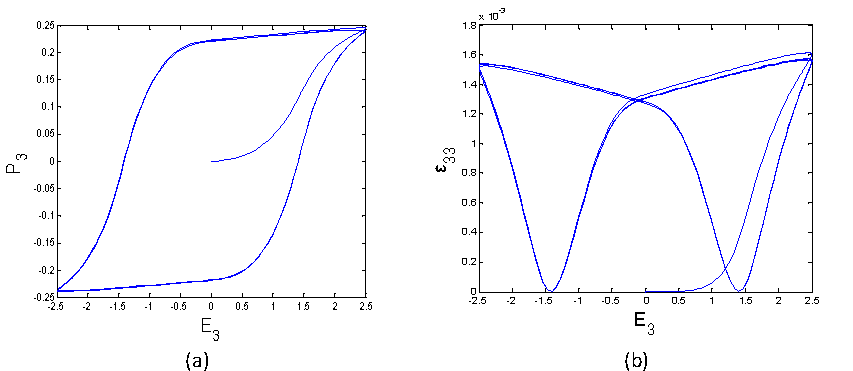
\includegraphics[width=5in]{./chap_2_pol_sw/figures/majorloop_polarization_switching.pdf}
\caption{Major hysteresis loops in a piezoelectric sample: a) polarization response and b) corresponding strain response}
\label{fig:Majorhysteresisloops}
\end{figure}
 
\begin{figure}
\centering
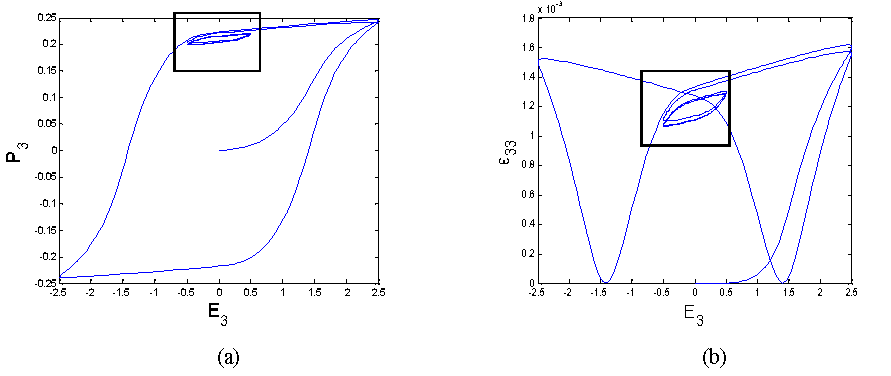
\includegraphics[width=5in]{./chap_2_pol_sw/figures/minorloop_polarization_switching.pdf}
\caption{Minor hysteresis loops in a polarized piezoelectric sample: a) polarization response and b) corresponding strain response}
\label{fig:Manorhysteresisloops}
\end{figure} 
  
\begin{figure}
\centering
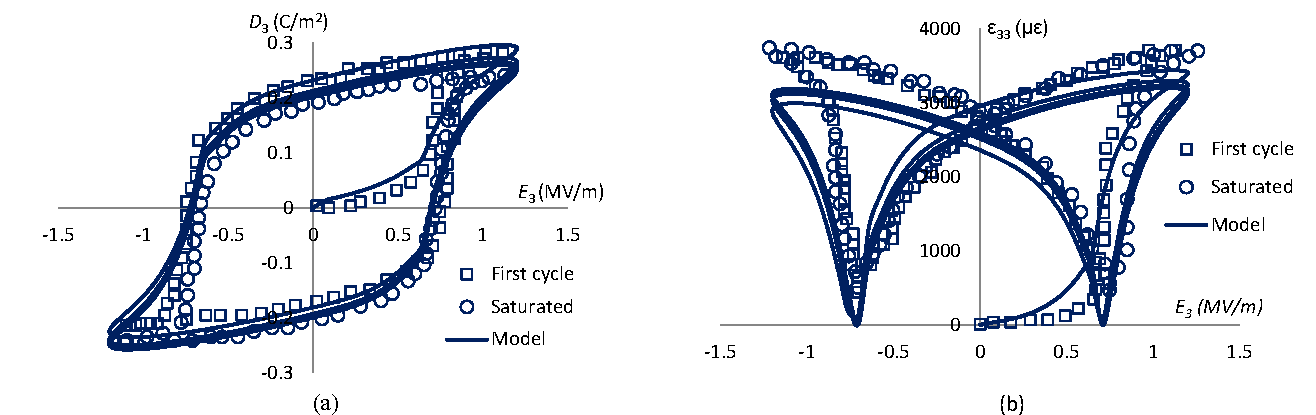
\includegraphics[width=5.0in]{./chap_2_pol_sw/figures/hysteresis_polarization_butterfly_strainres_ponsespzt_51_zero_stress.pdf}
\caption{Hysteresis polarization and butterfly strain responses for PZT51 at zero stress}
\label{fig:hysteresis_polarization_butterfly_strainres_ponsespzt_51_zerostress}
\end{figure}
  
\begin{figure} 
\centering
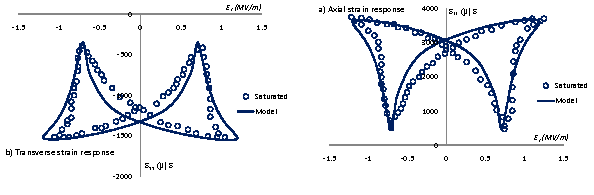
\includegraphics[width=5.0in]{./chap_2_pol_sw/figures/saturated_strain_responses_pzt51_zero_stress.pdf} 
\caption{Saturated strain responses for PZT51 at zero stress}
\label{saturated_strain_responses_pzt51_zero_stress}
\end{figure}

\begin{figure} 
\centering 
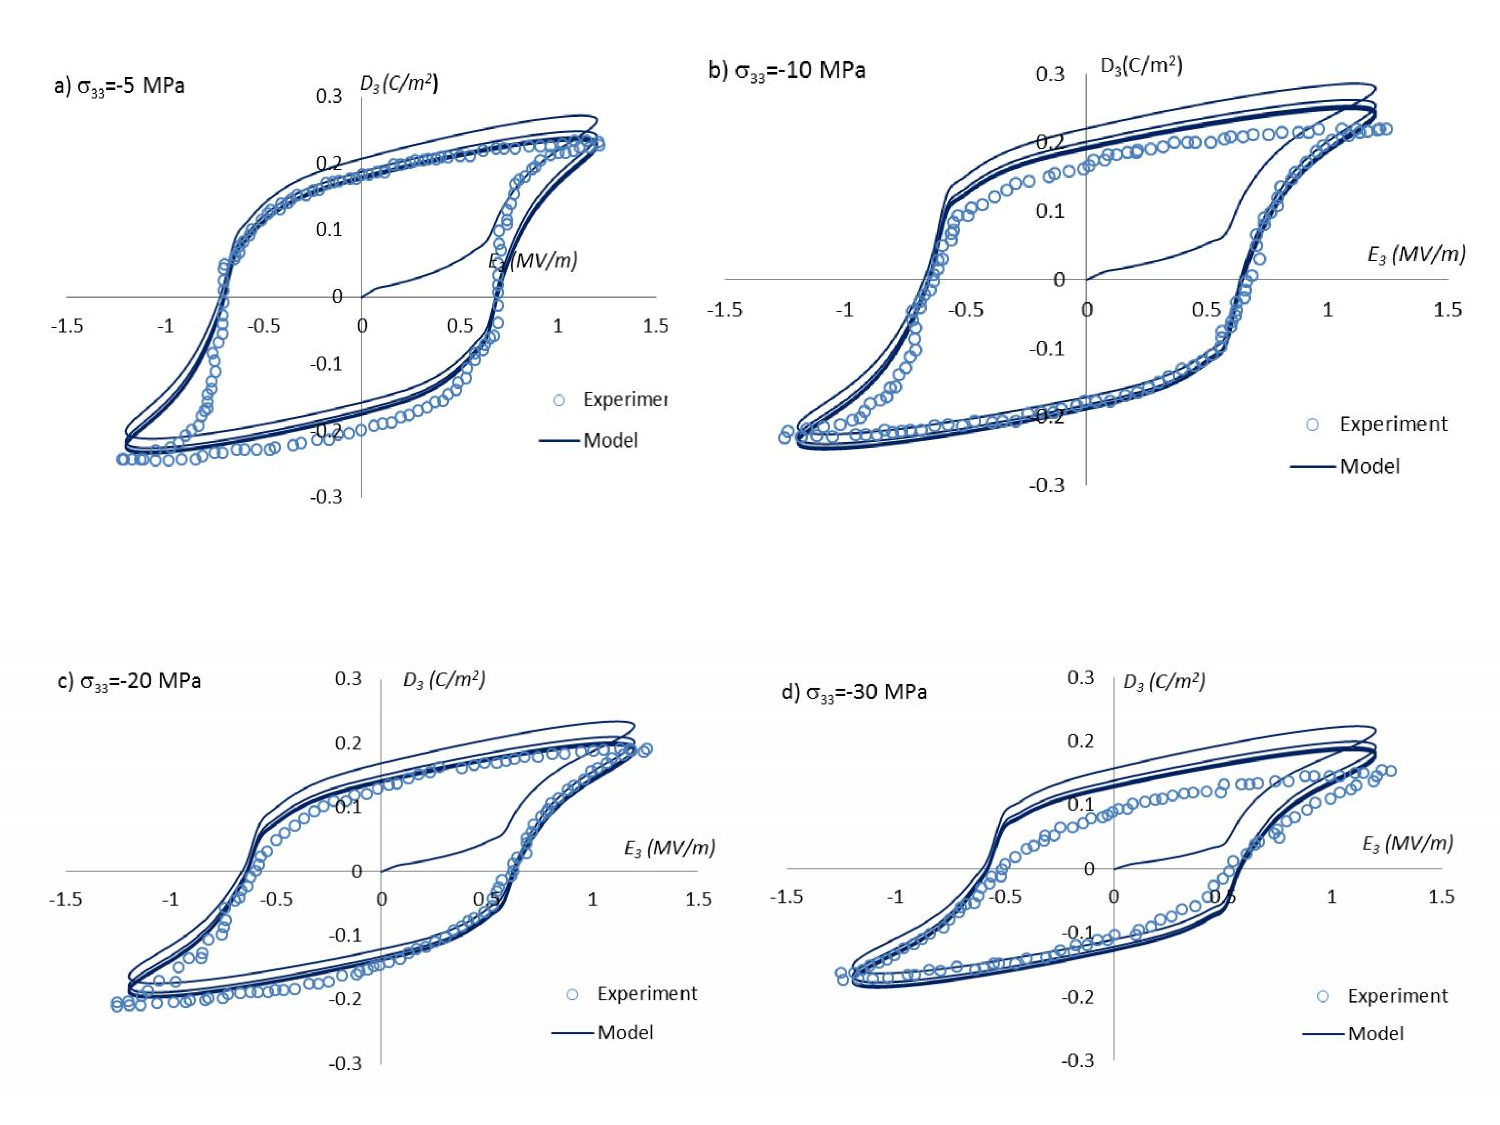
\includegraphics[width=5.0in]{./chap_2_pol_sw/figures/hysteresis_polarization_responses_under_constant_compressive_stresses.pdf} 
\caption{Hysteresis polarization responses under constant compressive stresses}
\label{hysteresis_polarization_responses_under_constant_compressive_stresses}
\end{figure}

\begin{figure}
\centering 
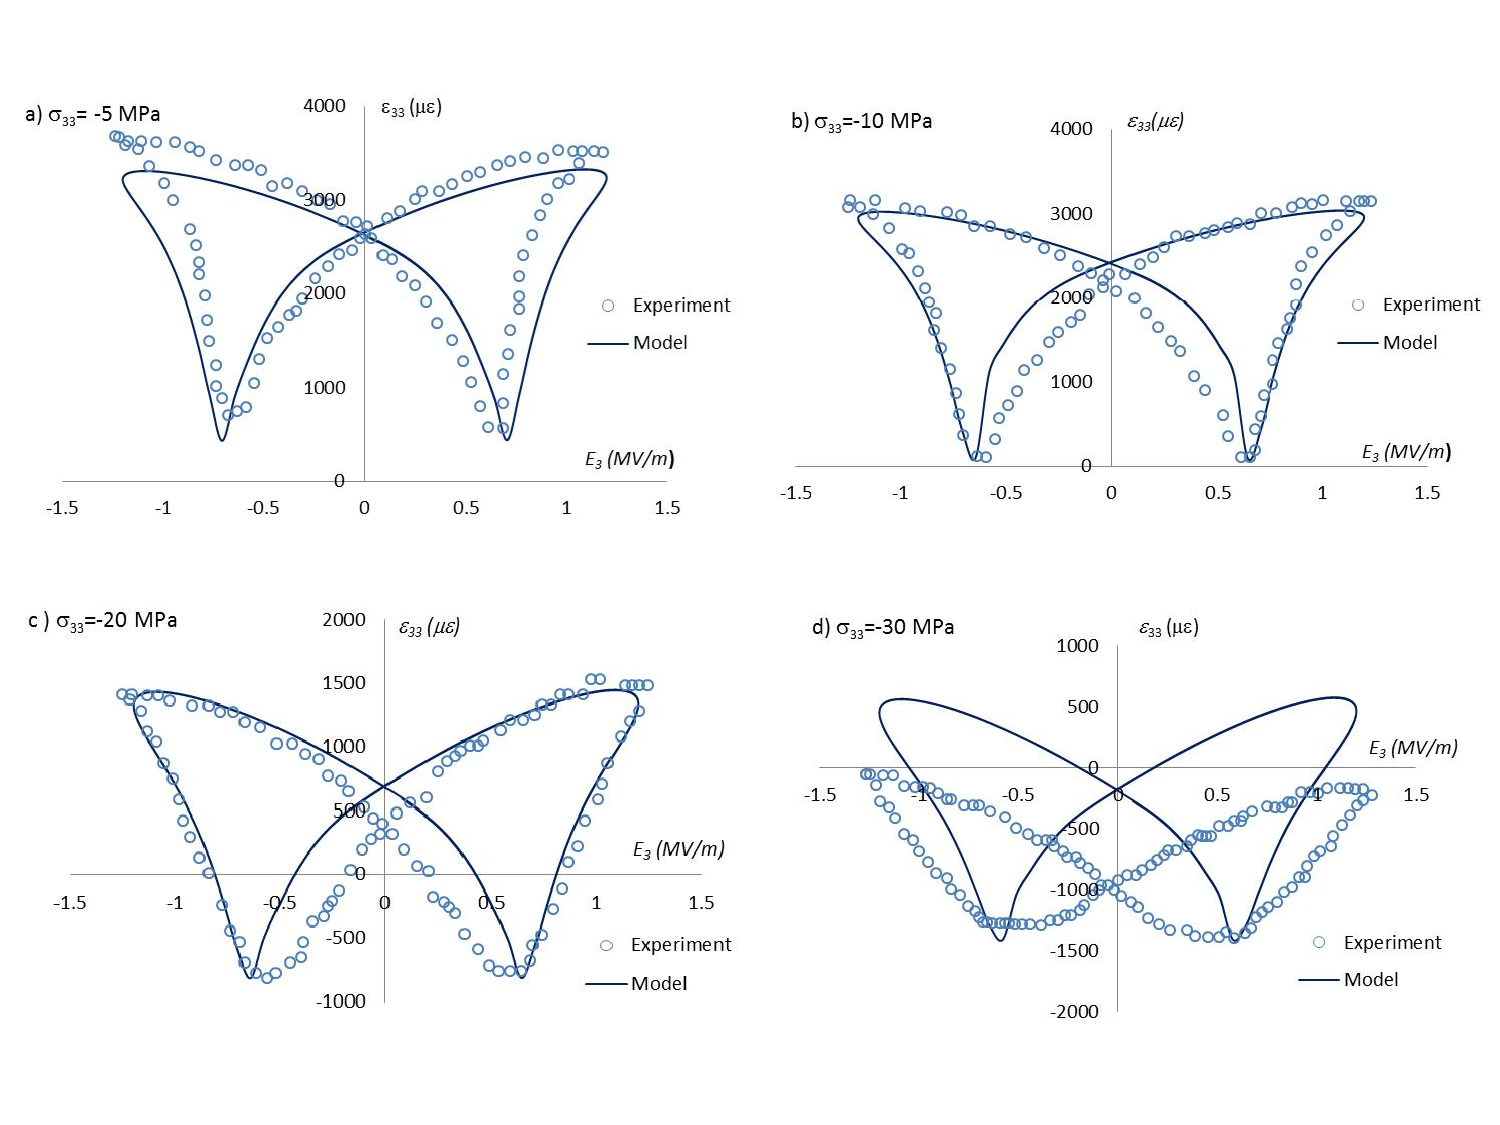
\includegraphics[width=5.0in]{./chap_2_pol_sw/figures/butterfly_strain_responses_under_constant_compressive_stresses.pdf} 
\caption{Butterfly strain responses under constant compressive stresses}
\label{butterfly_strain_responses_under_constant_compressive_stresses}
\end{figure}

\begin{figure} 
\centering 
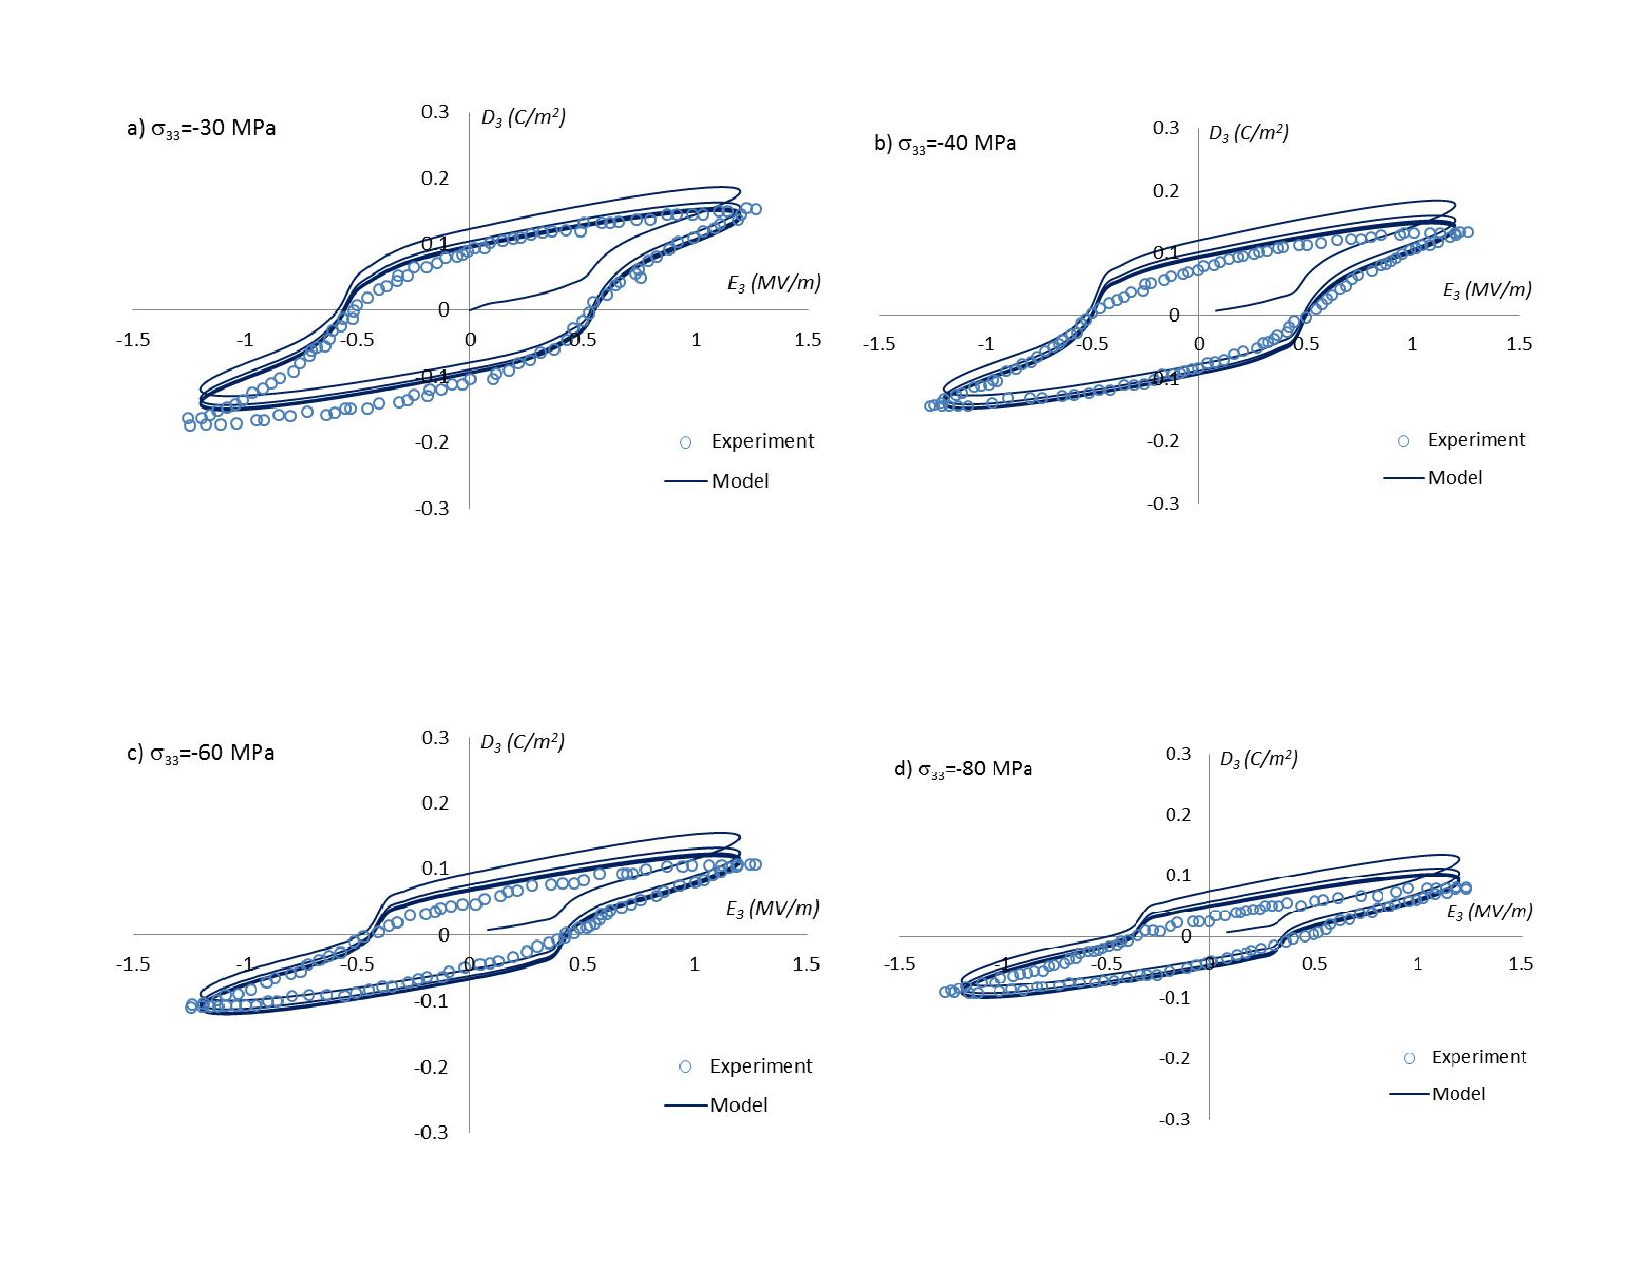
\includegraphics[width=5.0in]{./chap_2_pol_sw/figures/Fig_6_hysteresis_polarization_responses_under_constant_compressive_stresses_above_the_coercive_stress.pdf} 
\caption{Hysteresis polarization responses under constant compressive stresses above the coercive stress}
\label{Fig_6_hysteresis_polarization_responses_under_constant_compressive_stresses_above_the_coercive_stress}
\end{figure} 

\begin{figure} 
\centering 
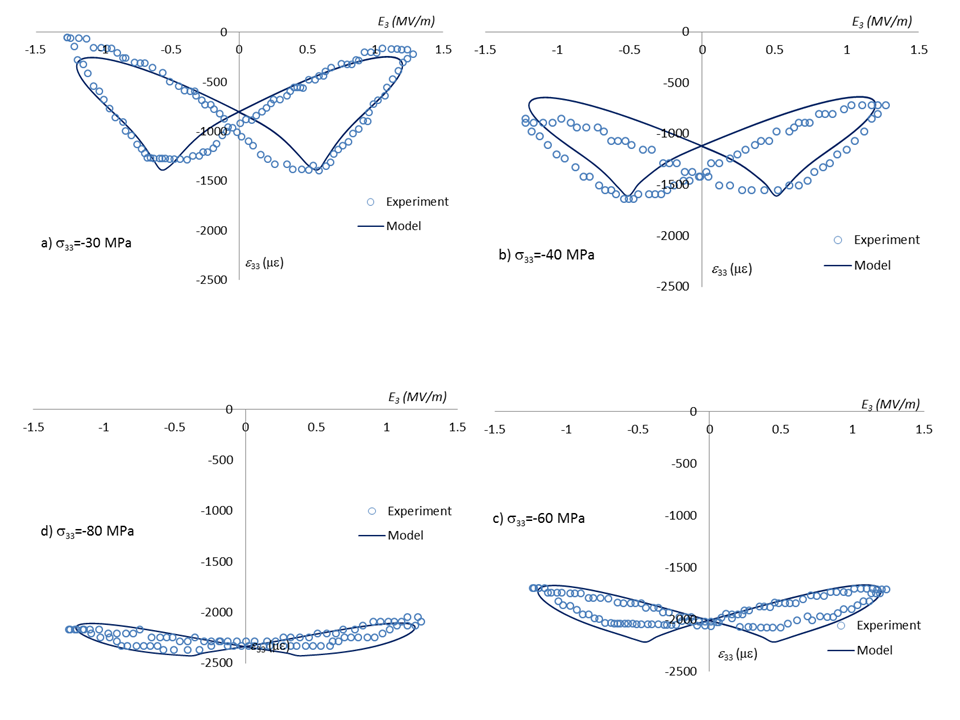
\includegraphics[width=5.0in]{./chap_2_pol_sw/figures/fig_7_butterfly_strain_responses_under_constant_compressive_stresses_above_the_coercive_stress.png} 
\caption{Butterfly strain responses under constant compressive stresses above the coercive stress}
\label{fig_7_butterfly_strain_responses_under_constant_compressive_stresses_above_the_coercive_stress}
\end{figure}

\begin{figure}
\centering
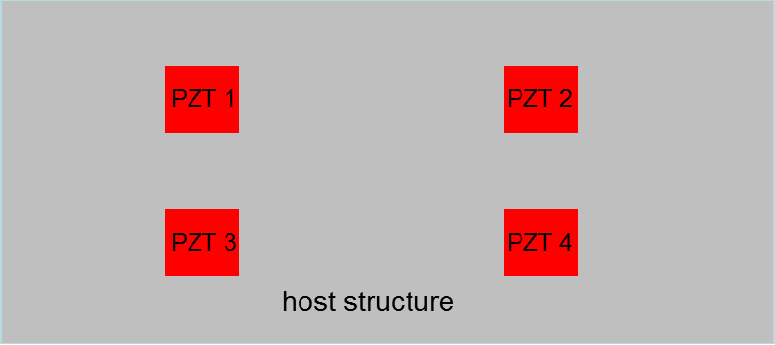
\includegraphics[width=5.0in]{./chap_2_pol_sw/figures/activecompositeplatewithpatches.pdf}
\caption{Active composite plate with PZT patches}
\label{fig:ActiveComposBeam} 
\end{figure}

\begin{figure}
\centering
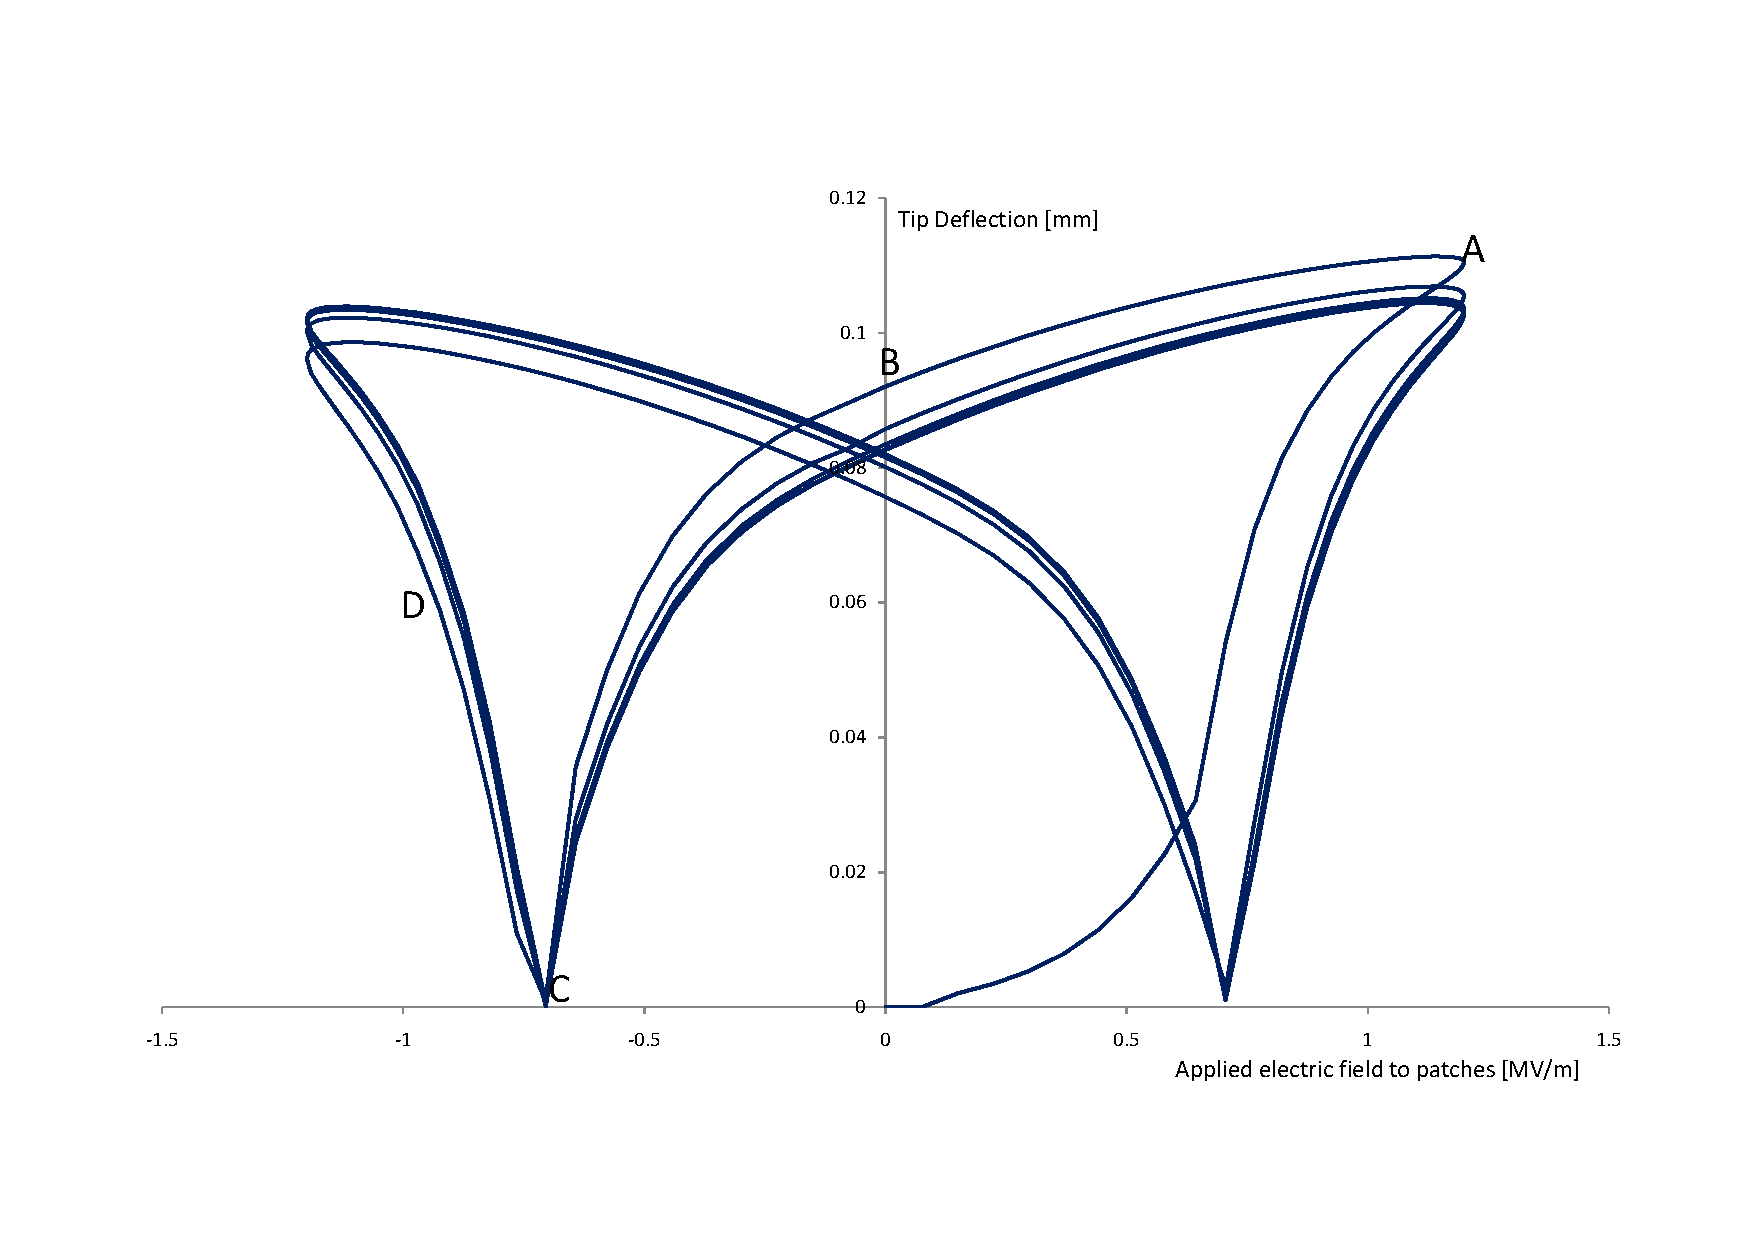
\includegraphics[width=5.0in]{./chap_2_pol_sw/figures/tipdeflectioncompositeactivebeam.pdf}
\caption{Tip deflection of the cantilever plate due to uniform cyclic electric fields applied to the piezoelectric patches}
\label{fig:tipdeflectioncompositeactivebeam}
\end{figure}
 
\begin{figure}
\centering
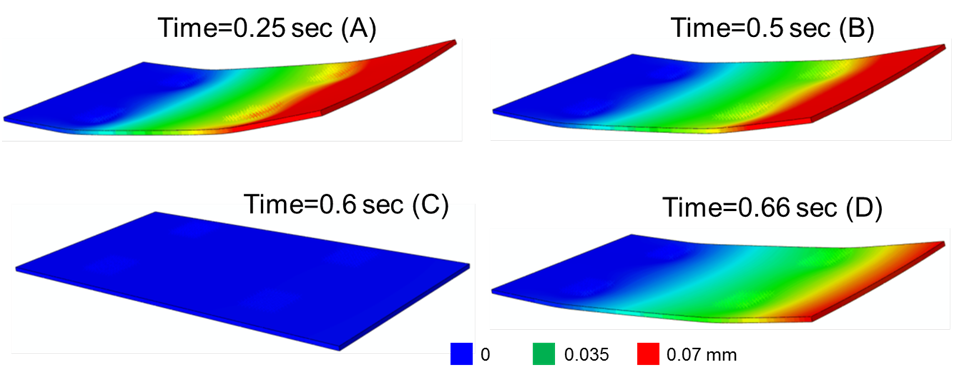
\includegraphics[width=5.0in]{./chap_2_pol_sw/figures/Figure_13_deformed_shape_active_cantilever.png}
\caption{The corresponding deformed shape of an active cantilever plate due to a uniform cyclic electric field applied to the piezoelectric patches}
\label{fig:Figure_13_deformed_shape_active_cantilever}
\end{figure}

\begin{figure} 
\centering
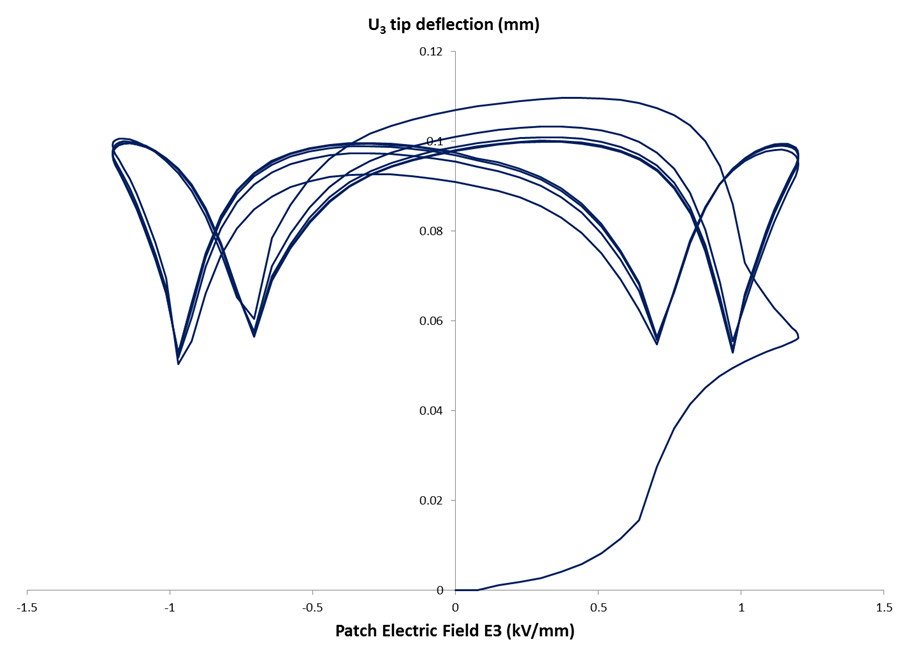
\includegraphics[width=5.0in]{./chap_2_pol_sw/figures/Fig14_tiptwistingcompositeactivebeam.png}
\caption{Tip deflection of the twisting cantilever plate due to a non-uniform cyclic electric field applied to the piezoelectric patches}
\label{fig:Fig14_tiptwistingcompositeactivebeam} 
\end{figure}

\begin{figure} 
\centering
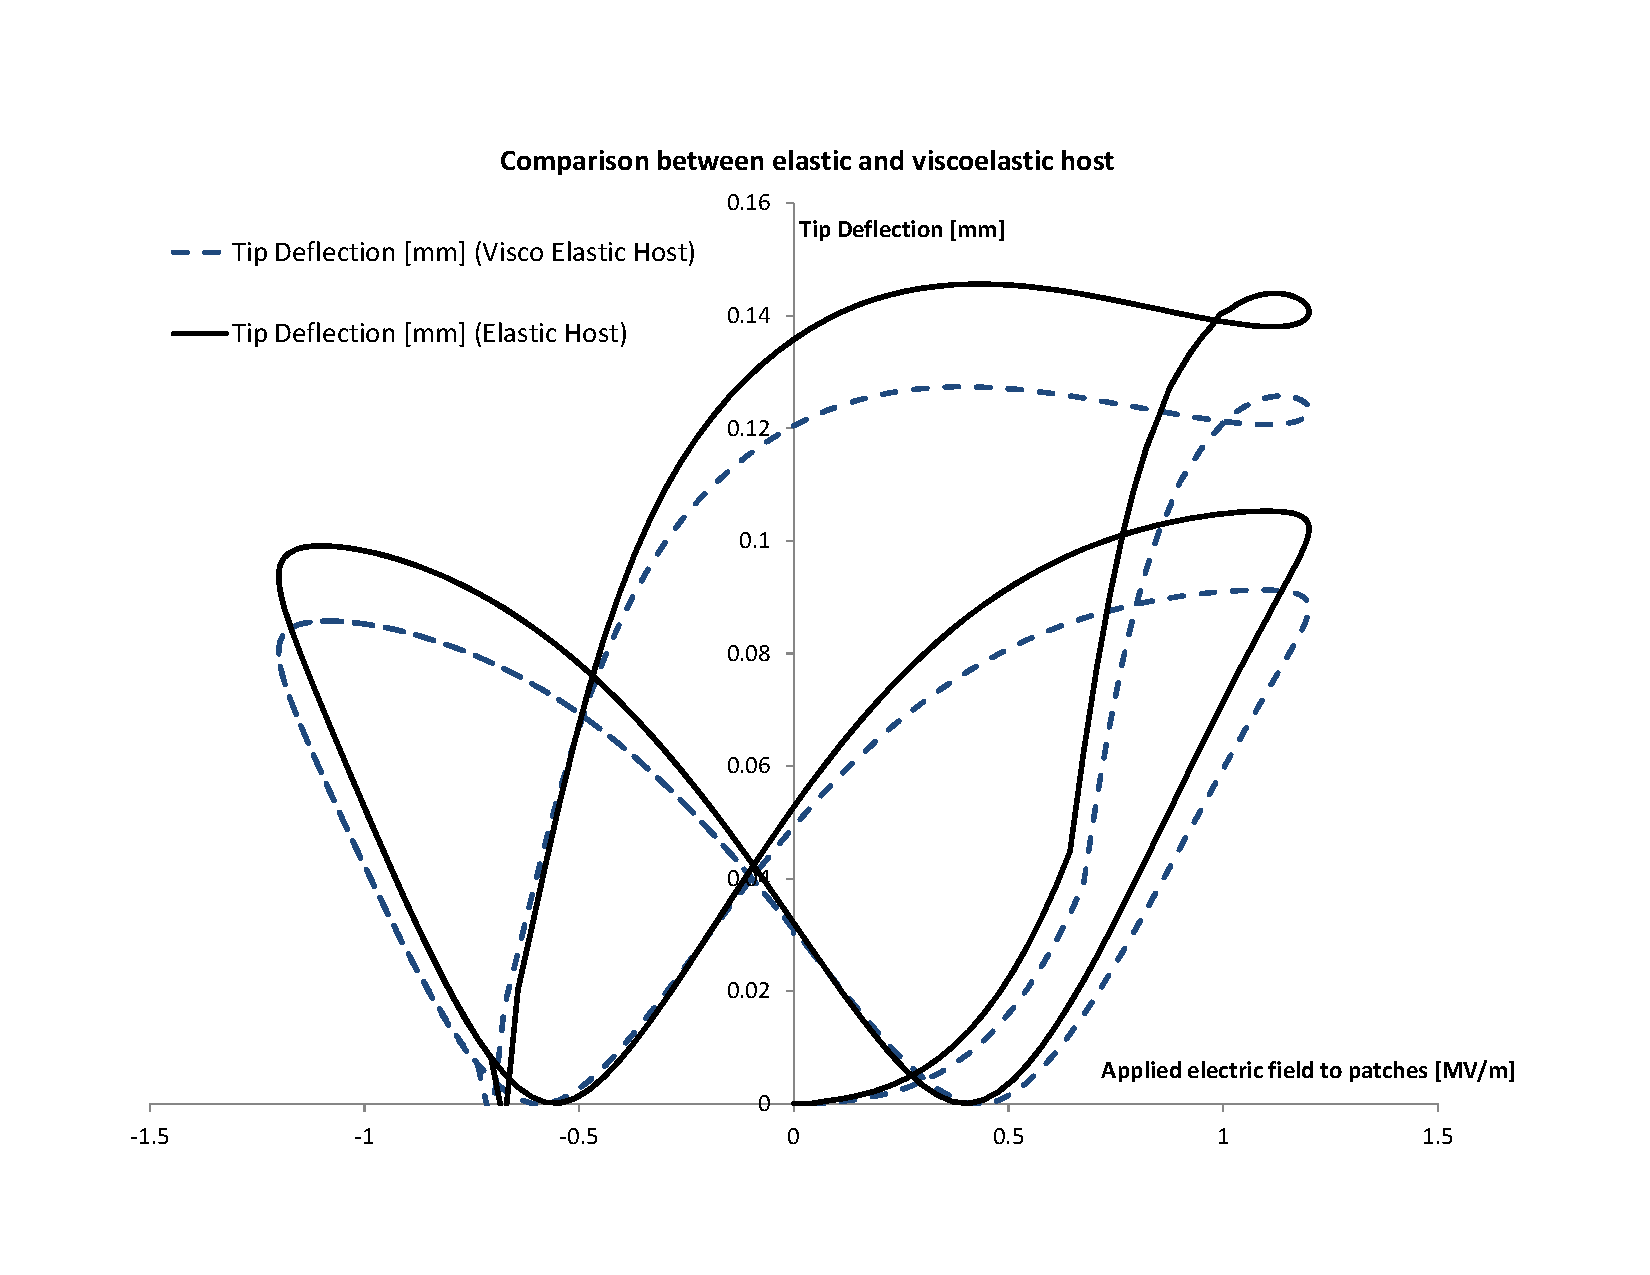
\includegraphics[width=5.0in]{./chap_2_pol_sw/figures/ViscoHostCompositeActiveBeam.pdf}
\caption{The comparison between viscoelastic and elastic materials as host structure}
\label{fig:ViscoHostCompositeActiveBeam}
\end{figure}

\newpage 